\section{Microvision ShowWX+ Spezifikationen}
\label{app:projector}
\begin{table}[!ht]
\caption{Spezifikationen des Microvision ShowWX+}
\begin{center}
\vspace{-3mm}
\begin{tabular}{|l|r|}
\hline
\rowcolor{lightgray} Eigenschaft & Spezifikation \\
\hline
Auflösung 	& WVGA (\SI{848}{}$\mathrm{x}$\SI{480}{}) \\
\hline
Seitenverhältnis & \SI{16}{}$:$\SI{9}{} \\
\hline
Helligkeit 	& \SI{15}{} Laser-Lumen \\
\hline
Wiederholfrequenz & \SI{60}{\Hz} \\
\hline
Farbumfang 	& $\sim$ \SI{200}{}\% NTSC \\
\hline
Kontrastverhältnis 	& $>$ \SI{5.000}{}$:$\SI{1}{} \\
\hline
Projektionsverhältnis 	& \SI{1}{}$:$\SI{1}{} \\
\hline
Öffnungswinkel & $\sim$ \SI{30}{°}\\
\hline
Projektionsdistanz 	& \SI{200}{\milli\meter}$-$\SI{2500}{\milli\meter} \\
\hline
Bildgröße 	& \SI{150}{\milli\meter}$-$\SI{2500}{\milli\meter} \\
\hline
Verschlüsselung 	& HDCP \\
\hline
Videoeingang & HDMI (\SI{480}{p}) \\
\hline
Gewicht 	& \SI{122}{\gram} \\
\hline
\end{tabular}
\end{center}
\label{tab:landmarks_f1}
\end{table}

\begin{figure}[hb]
\vspace{-5mm}
\begin{center}
		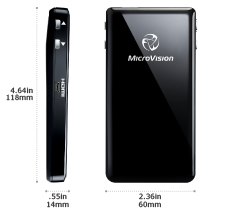
\includegraphics[scale=0.8]{measurements_showwx}
\end{center}
\vspace{-5mm}
\caption{Abmessungen des Microvision ShowWX+}
\label{fig.specs_proj}
\end{figure}

\clearpage{}

\section{Technische Spezifikationen des Arduino Nano}
\label{app:arduino}

\begin{table}[ht]
\caption{Technische Spezifikationen des Arduino Nano}
\begin{center}
\begin{tabular}{|l|r|}
\hline
\rowcolor{lightgray} \multicolumn{1}{|c|}{\textbf{Spezifikation}} & \multicolumn{1}{|c|}{\textbf{Wert}}\\
\hline
Microcontroller & Atmel ATmega328\\
\hline
Betriebsspannung & \SI{5}{\volt}\\
\hline
Eingangsspannung & \SI{7}{}$-$\SI{12}{\volt}\\
\hline
Grenzen der Eingangsspannung & \SI{6}{}$-$\SI{20}{\volt}\\
\hline
Digitale I/O Pins & \SI{14}{}\\
\hline
Analoge Eingangspins & \SI{8}{}\\
\hline
Gleichstrom pro I/O Pin & \SI{40}{\milli\ampere}\\
\hline
Flash Speicher & \SI{32}{KB}\\
\hline
SRAM & \SI{2}{KB} \\
\hline
EEPROM & \SI{1}{KB}\\
\hline
Taktfrequenz & \SI{16}{\mega\Hz}\\
\hline
Länge & \SI{45}{\milli\meter}\\
\hline
Breite & \SI{18}{\milli\meter}\\
\hline
Gewicht & \SI{5}{\gram}\\
\hline
\end{tabular}
\end{center}
\label{tab:arduino}
\end{table}

\clearpage{}

\section{Technische Spezifikationen des Raspberry Pi}
\label{app:raspberry}

\begin{table}[ht]
\caption{Technische Spezifikationen des Raspberry Pi}
\begin{center}
\begin{tabular}{|l|r|}
\hline
\rowcolor{lightgray} \multicolumn{1}{|c|}{\textbf{Spezifikation}} & \multicolumn{1}{|c|}{\textbf{Wert}}\\
\hline
System-on-a-Chip & Broadcom BCM2835\\
\hline
CPU & \SI{700}{\mega\Hz} ARM11 ARM1176JZF-S\\
\hline
GPU & Broadcom VideoCore IV\\
\hline
Speicher & \SI{512}{GB}\\
\hline
USB 2.0 Ports & \SI{2}{}\\
\hline
Videoausgänge & Composite RCA, HDMI\\
\hline
Audioausgänge & \SI{3,5}{\milli\meter} Jack, HDMI\\
\hline
Low-Level Peripherie & \SI{26}{} General Purpose Input/Output Pins,\\
& Serial Peripheral Bus Interface (SPI), I²C, I²S,\\
& Universal Asynchronous receiver/transmitter (UART)\\
\hline
Netzwerkschnittstelle & \SI{10}{}/\SI{100}{} wired Ethernet RJ45\\
\hline
Stromaufnahme & \SI{700}{\milli\ampere}\\
\hline
Spannungsversorgung & \SI{5}{\volt}\\
\hline
Länge & \SI{85}{\milli\meter}\\
\hline
Breite & \SI{56}{\milli\meter}\\
\hline
Höhe & \SI{15}{\milli\meter}\\
\hline
Gewicht & \SI{31}{\gram}\\
\hline
\end{tabular}
\end{center}
\label{tab:raspberry}
\end{table}

\clearpage{}

\section{Technische Spezifikationen der inertialen Messeinheit}
\label{app.imu}

\begin{table}[ht]
\caption{Technische Spezifikationen des Raspberry Pi}
\begin{center}
\begin{tabular}{|l|r|}
\hline
\rowcolor{lightgray} \multicolumn{1}{|c|}{\textbf{Spezifikation}} & \multicolumn{1}{|c|}{\textbf{Wert}}\\
\hline
Typ & MPU-9250 \\
\hline
Stromaufnahme & \SI{3,5}{\milli\ampere} \\
\hline
Spannungsversorgung & \SI{2,4}{}$-$\SI{3,6}{\volt} \\
\hline
Schnittstellen & I²C, SPI \\
\hline
Messbereich Drehrate & \SI{250}{}$-$\SI{2000}{} $\nicefrac{\deg}{\sec}$\\
\hline
Messbereich Beschleunigung &  \SI{2}{}$-$\SI{16}{} $\mathrm{g}$\\
\hline
Breite & \SI{20}{\milli\meter} \\
\hline
Höhe & \SI{22}{\milli\meter}\\
\hline
\end{tabular}
\end{center}
\label{tab:raspberry}
\end{table}

\clearpage{}

\section{Datenstruktur zur Repräsentation der Modellszene}
\label{app.datastructure}
\begin{lstlisting}[label=source.data,caption=Datenstruktur zur Repräsentation der Modellszene]
<?xml version="1.0"?>
<modelscene>
     <name>Model World</name>
     <object>
          <name>Map</name>
          <position>
          	<x> 0 </x>
          	<y> 0 </y>
          	<z> 0 </z>
          </position>
          <orientation>
          	<x> 0 </x>
          	<y> 0 </y>
          	<z> 0 </z>
          </orientation>
          <texture> map.jpg </texture>
          <geometry> map.obj </geometry>
     </object>
          <object>
          <name>Power Outlet</name>
          <position>
          	<x> 3.15 </x>
          	<y> 1.8 </y>
          	<z> 0.4 </z>
          </position>
          <orientation>
          	<x> 90 </x>
          	<y> 0 </y>
          	<z> 180 </z>
          </orientation>
          <texture> outlet.jpg </texture>
          <geometry> outlet.obj </geometry>
     </object>
</modelscene>
\end{lstlisting}

\clearpage{}

%\section{Bayes Filter}
%\label{app:bayes}
%
%\clearpage{}

\section{Konstruktionszeichnungen und Modelle}
\label{app:construction}

\clearpage{}

\section{Launchfiles}
\label{app:launchfiles}